\documentclass[aspectratio=169]{beamer}
\usepackage{will_handley_beamer}
\usepackage{title_page}

% Commands
% --------
% - \arxiv{arxiv number}
% - \arxiv{<number>}            arxiv.org/abs/<number>
% - \oldarxiv{<arxiv number>}   arxiv.org/<number>
% - \doi{<doi>}                 doi.org/<doi>
% - \xkcd{<number>}             xkcd.com/<number>
% - \email{<email>}             <<email>>
% - \tthref{<website>}          <website>
% - \av[dist]{<quantity>}       <quantity>_{dist}
% - \student{<name>}{<detail>}{<photo>}

% Talk details
% ------------
\title{\texttt{lsbi}: linear simulation based inference }
\subtitle{\arxiv{2501.03921}}
\date{19\textsuperscript{th} July 2025}

\begin{document}

\begin{frame}
    \titlepage
\end{frame}

\begin{frame}
    \begin{quote}
        ``If asked what is the most under-used Machine Learning technique in physics\ldots\\ \hfill\ldots my answer is only half-jokingly \textbf{linear regression}.''\hspace{20pt} 
    \end{quote}

    \hfill Jesse Thaler [phystat 2024]
\end{frame}

\begin{frame}
    \frametitle{Who?}
    \begin{columns}
        \column{0.8\textwidth}
        Idea I've been working on/talking about on-and-off for the better part of 2 years,
        \begin{itemize}
            \item Nicolas Mediato Diaz (MSci project)
            \item David Yallup (Postdoc)
            \item Thomas Gessey Jones (Postdoc)
            \item Toby Lovick (PhD student)
        \end{itemize}

        Many others have also presented this idea independently
        \begin{itemize}
            \item \texttt{SELFI} incorporates much of this idea: Leclercq~\arxiv{1902.10149}
            \item some of these ideas are in \texttt{MOPED}: Heavens~\oldarxiv{astro-ph/9911102}
            \item Also appears in Häggström~\arxiv{2403.07454}
        \end{itemize}

        \column{0.14\textwidth}
        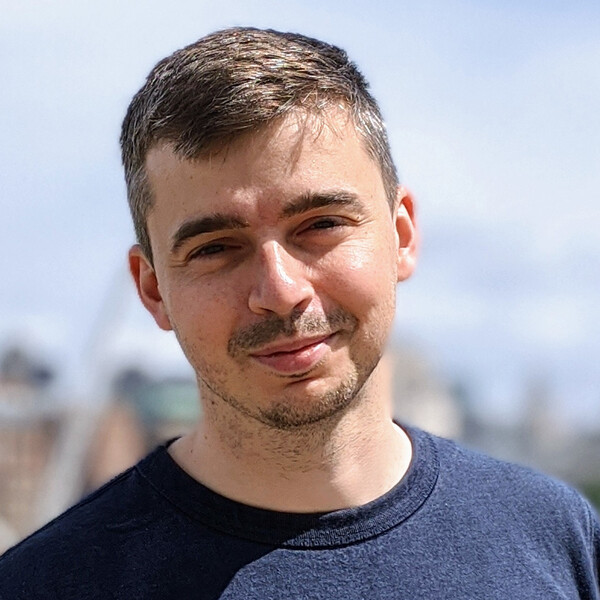
\includegraphics[width=\textwidth]{people/david_yallup}
\tiny{David Yallup}

        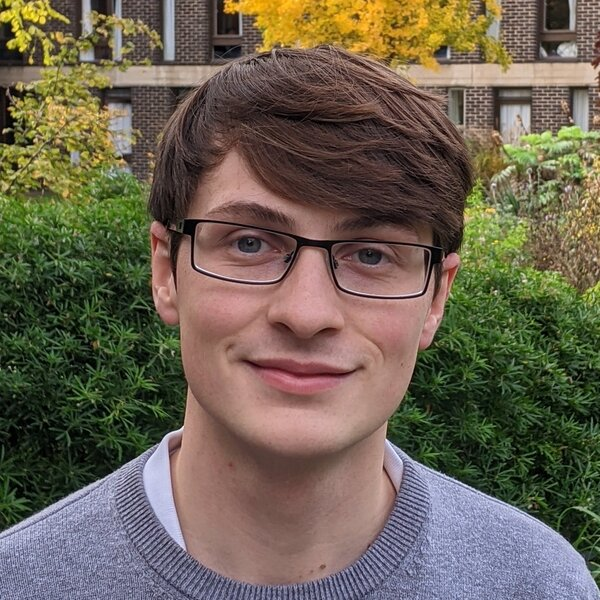
\includegraphics[width=\textwidth]{people/thomas_gessey-jones}
\tiny{Thomas Gessey-Jones}

        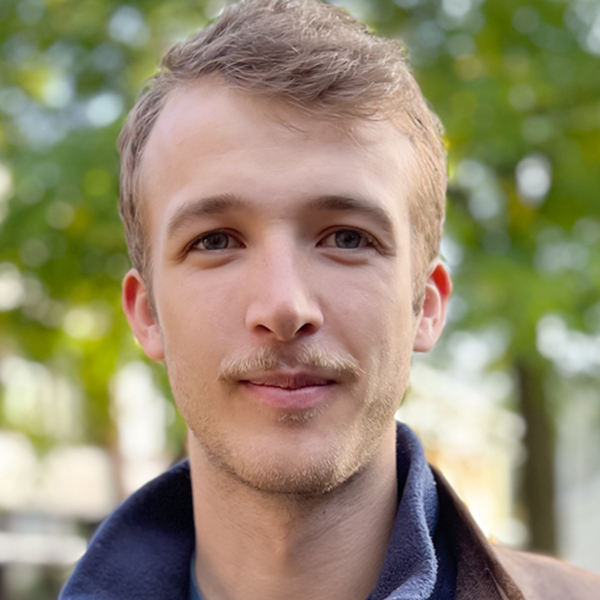
\includegraphics[width=\textwidth]{people/toby_lovick}
\tiny{Toby Lovick}

    \end{columns}
\end{frame}

\begin{frame}
    \frametitle{SBI: Simulation-based inference}
    \begin{columns}
        \column{0.5\textwidth}
        \begin{itemize}
            \item What do you do if you don't know \C[2]{$\mathcal{L}(D|\theta)$}?
            \item If you have a simulator/forward model $\theta \rightarrow D$
                defines an \C[2]{\emph{implicit} likelihood~$\mathcal{L}$}.
            \item Simulator generates samples from $\C[2]{\mathcal{L}(\cdot|\theta)}$.
            \item With a \C[1]{prior $\pi(\theta)$} can generate samples from \C[4]{joint distribution}~$\C[4]{\mathcal{J}(\theta,D)}=\C[2]{\mathcal{L}(D|\theta)}\C[1]{\pi(\theta)}$\\\hfill \emph{the ``probability of everything''}.
            \item Task of SBI is take joint~$\C[4]{\mathcal{J}}$ samples and learn \C[0]{posterior $\mathcal{P}(\theta|D)$},  and \C[3]{evidence $\mathcal{Z}(D)$} \\ or even \C[2]{likelihood~$\mathcal{L}(D|\theta)$} or \C[4]{joint~$\mathcal{J}(\theta,D)$}.
            \item Present state of the art achieves this using \emph{machine learning} (neural networks).
        \end{itemize}
        \column{0.5\textwidth}
        \includegraphics<1|handout:0>[page=1, width=\textwidth]{figures/sbi_parameter_estimation.pdf}%
        \includegraphics<2|handout:0>[page=2, width=\textwidth]{figures/sbi_parameter_estimation.pdf}%
        \includegraphics<3|handout:0>[page=3, width=\textwidth]{figures/sbi_parameter_estimation.pdf}%
        \includegraphics<4|handout:0>[page=4, width=\textwidth]{figures/sbi_parameter_estimation.pdf}%
        \includegraphics<5|handout:0>[page=5, width=\textwidth]{figures/sbi_parameter_estimation.pdf}%
        \includegraphics<6|handout:0>[page=6, width=\textwidth]{figures/sbi_parameter_estimation.pdf}%
        \includegraphics<7|handout:0>[page=7, width=\textwidth]{figures/sbi_parameter_estimation.pdf}%
        \includegraphics<8|handout:0>[page=8, width=\textwidth]{figures/sbi_parameter_estimation.pdf}%
        \includegraphics<9|handout:0>[page=9, width=\textwidth]{figures/sbi_parameter_estimation.pdf}%
        \includegraphics<10|handout:0>[page=10, width=\textwidth]{figures/sbi_parameter_estimation.pdf}%
        \includegraphics<11|handout:0>[page=11, width=\textwidth]{figures/sbi_parameter_estimation.pdf}%
        \includegraphics<12|handout:0>[page=12, width=\textwidth]{figures/sbi_parameter_estimation.pdf}%
        \includegraphics<13|handout:0>[page=13, width=\textwidth]{figures/sbi_parameter_estimation.pdf}%
        \includegraphics<14|handout:0>[page=14, width=\textwidth]{figures/sbi_parameter_estimation.pdf}%
        \includegraphics<15|handout:0>[page=15, width=\textwidth]{figures/sbi_parameter_estimation.pdf}%
        \includegraphics<16|handout:0>[page=16, width=\textwidth]{figures/sbi_parameter_estimation.pdf}%
        \includegraphics<17|handout:0>[page=17, width=\textwidth]{figures/sbi_parameter_estimation.pdf}%
        \includegraphics<18|handout:0>[page=18, width=\textwidth]{figures/sbi_parameter_estimation.pdf}%
        \includegraphics<19|handout:0>[page=19, width=\textwidth]{figures/sbi_parameter_estimation.pdf}%
        \includegraphics<20|handout:0>[page=20, width=\textwidth]{figures/sbi_parameter_estimation.pdf}%
        \includegraphics<21>[page=21, width=\textwidth]{figures/sbi_parameter_estimation.pdf}%
    \end{columns}
\end{frame}

\begin{frame}
    \frametitle{Why \textit{linear} SBI?}
    If neural networks are all that, why should we consider the regressive step of going back to linear versions of this problem?

    \begin{itemize}
        \item It is pedagogically helpful 
            \begin{itemize}
                \item separates general principles of SBI from the details of neural networks
                \item (particularly for ML skeptics)
            \end{itemize}
        \item It is practically useful
            \begin{itemize}
                \item for producing expressive examples with known ground truths. 
            \end{itemize}
        \item It is pragmatically useful
            \begin{itemize}
                \item competitive with neural approaches in terms of accuracy,
                \item faster and more interpretable. 
            \end{itemize}
    \end{itemize}
\end{frame}

\begin{frame}
    \frametitle{Linear Simulation Based Inference}
    \framesubtitle{Mathematical setup}
    \begin{columns}[t]
        \column{0.5\textwidth}
        \begin{itemize}
            \item Linear generative model $(m,M,C)$
                \[ 
                    \only<1>{D = m + M \theta \pm \sqrt{C}}%
                    \only<2->{D \sim \mathcal{N}(m + M \theta, C)}%D \sim 
                \]
                where:
                \begin{description}
                    \item[$\theta$]: $n$ dimensional parameters
                    \item[$D$]: $d$ dimensional data
                    \item[$M$]: $d\times n$ transfer matrix
                    \item[$m$]: $d$-dimensional shift
                    \item[$C$]:  $d\times d$ data covariance
                \end{description}
        \end{itemize}

        \column{0.5\textwidth}
        \only<3->{
        \begin{itemize}
            \item $k$ Simulations 
                \[
                    S=\{ (\theta_i,D_i): i=1,\ldots,k\}
                \]
            \item Define simulation statistics\footnotemark:

                \begin{description}
                    \item[$\bar\theta$] $= \tfrac{1}{k}\sum_k \theta_i$
                    \item[$\bar D$] $= \tfrac{1}{k}\sum_k D_i$
                    \item[$\Theta$] $=\tfrac{1}{k}\sum_i (\theta_i-\bar\theta)(\theta_i-\bar\theta)'$
                    \item[$\Delta$] $=\tfrac{1}{k}\sum_i (D_i-\bar D)(D_i-\bar D)'$
                    \item[$\Psi$] $=\tfrac{1}{k}\sum_i (D_i-\bar D)(\theta_i-\bar \theta)'$
                \end{description}
        \end{itemize}
    }
    \end{columns}
    \footnotetext[1]{N.B. using matrix variate notation where primes denote transposes $M' = M^T$}
\end{frame}

\begin{frame}
    \frametitle{Gory mathematical details}
    \student{toby_lovick}{PhD student}{Toby Lovick}
    \begin{columns}
        \column{0.55\textwidth}
        \begin{itemize}
            \item We now wish to infer the parameters of the linear model $(m,M,C)$ from simulations $S$ \linebreak (which define $\bar\theta,\bar D, \Theta, \Delta, \Psi$)
            \item The likelihood for this problem is:
                \begin{align*}
                    \C[2]{\mathcal{L}(M,m,c)} &= P(\{D_i\}|\{\theta_i\}|m, M, C) \\
                &= \prod_i \mathcal{N}(D_i|m+M\theta_i,C)
\end{align*}
                \onslide<2->{
                    \vspace{-15pt}
            \item It can be shown the \C[1]{prior $\pi$} and  \C[0]{posterior $\mathcal{P}$} are conjugately\ldots
        \begin{align*}
            m&|M,C, \sim \mathcal{N}(D_p-M\theta_p, \tfrac{1}{\lambda_p}C), \\
            M&|C, \sim \mathcal{MN}(M_p, C, \Omega_p^{-1}), \\
            C &\sim \mathcal{W}^{-1}_{\nu_p}(\Psi_p)
        \end{align*}
                }
        \end{itemize}

        \column{0.45\textwidth}
        \hfill\includegraphics<2>[width=0.7\textwidth]{figures/matrix_variate_distributions.jpg}%
    \only<3->{
        \small{
\begin{align}
\nu_\mathcal{P} =& \nu_\pi+k,\qquad \lambda_\mathcal{P} = \lambda_\pi+k\qquad\nonumber\\
\theta_\mathcal{P} =& \frac{\lambda_\pi\theta_\pi + k\bar{\theta}}{\lambda_\pi+k}\qquad
D_\mathcal{P} = \frac{\lambda_\pi D_\pi + k\bar{D}}{\lambda_\pi+k}\nonumber\\
\Omega_\mathcal{P} =&  \Omega_\pi+ k\Theta + \tfrac{k\lambda_\pi}{k+\lambda_\pi}(\theta_\pi-\bar{\theta})(\theta_\pi-\bar{\theta})'\nonumber\\
M_\mathcal{P}\Omega_\mathcal{P} =& M_\pi \Omega_\pi + k \Phi \nonumber\\
&+ \tfrac{k\lambda_\pi}{k+\lambda_\pi}(D_\pi-\bar{D})(\theta_\pi-\bar{\theta})', \nonumber\\
    \Psi_\mathcal{P} =&\Psi_\pi + k\Delta-k\Phi\Theta^{-1}\Phi' \nonumber\\
    &+\tfrac{k\lambda_\pi}{k+\lambda_\pi} (M_\mathcal{P}(\theta_\pi-\bar{\theta}) - (D_\pi-\bar{D})) \nonumber\\
    &\hspace{35pt}(M_\mathcal{P}(\theta_\pi-\bar{\theta})- (D_\pi-\bar{D}))'  \nonumber\\
    &+ k(M_\mathcal{P}-\Phi\Theta^{-1})\Theta(M_\mathcal{P}-\Phi\Theta^{-1})' \nonumber\\
    &+(M_\mathcal{P}-M_\pi)\Omega_\pi(M_\mathcal{P}-M_\pi)' \nonumber
\end{align}
}
}
    \end{columns}
\end{frame}

\begin{frame}
    \frametitle{Sequential LSBI}
    \begin{itemize}
        \item As we shall see, for non-linear problems, a linear approximation is unlikely to be a good one.
        \item Sequential methods iteratively improve by focussing effort around observed data~$D_\text{obs}$.
            \begin{itemize}
                \item This is orthogonal to amortised approaches
                \item More appropriate to cosmology, where there is only one dataset
                \item Less appropriate to particle physics/GW
            \end{itemize}
        \item We are free to choose where to place simulation parameters $\{\theta_i\}$, so it makes sense to choose these so that they generate simulations close to the observed data
        \item Our current approximation to the posterior is a natural choice.
    \end{itemize}
\end{frame}

\begin{frame}
    \frametitle{Example of this on our toy model}
    \student{toby_lovick}{PhD student}{Toby Lovick}
    \begin{columns}
        \column{0.5\textwidth}
        \begin{itemize}
            \item<1-> Same model as before
            \item<2-> Mark the observed data~$D_\text{obs}$
            \item<3-> Fit a model using \texttt{lsbi}
            \item<4-> Evaluate the posterior (cheap as linear)
            \item<5-> Now use this posterior to pick $\{\theta_i\}$
            \item<5-> Generate $\{D_i\}$ from original simulator
            \item<6-> Fit \texttt{lsbi} to these
            \item<7-> Evaluate the new posterior
            \item<8-> Iterate
        \end{itemize}

        \column{0.5\textwidth}
        \includegraphics<1|handout:0>[width=\textwidth, page=1]{figures/lsbi_plot.pdf}%
        \includegraphics<2|handout:0>[width=\textwidth, page=2]{figures/lsbi_plot.pdf}%
        \includegraphics<3|handout:0>[width=\textwidth, page=3]{figures/lsbi_plot.pdf}%
        \includegraphics<4|handout:0>[width=\textwidth, page=4]{figures/lsbi_plot.pdf}%
        \includegraphics<5|handout:0>[width=\textwidth, page=5]{figures/lsbi_plot.pdf}%
        \includegraphics<6|handout:0>[width=\textwidth, page=6]{figures/lsbi_plot.pdf}%
        \includegraphics<7|handout:0>[width=\textwidth, page=7]{figures/lsbi_plot.pdf}%
        \includegraphics<8|handout:0>[width=\textwidth, page=8]{figures/lsbi_plot.pdf}%
        \includegraphics<9|handout:0>[width=\textwidth, page=9]{figures/lsbi_plot.pdf}%
        \includegraphics<10|handout:0>[width=\textwidth, page=10]{figures/lsbi_plot.pdf}%
        \includegraphics<11|handout:0>[width=\textwidth, page=11]{figures/lsbi_plot.pdf}%
        \includegraphics<12|handout:0>[width=\textwidth, page=12]{figures/lsbi_plot.pdf}%
        \includegraphics<13|handout:0>[width=\textwidth, page=13]{figures/lsbi_plot.pdf}%
        \includegraphics<14|handout:0>[width=\textwidth, page=14]{figures/lsbi_plot.pdf}%
        \includegraphics<15|handout:0>[width=\textwidth, page=15]{figures/lsbi_plot.pdf}%
        \includegraphics<16>[width=\textwidth, page=16]{figures/lsbi_plot.pdf}%
    \end{columns}
\end{frame}

\begin{frame}
    \frametitle{Example of this on the CMB~\arxiv{2501.03921}}
    \begin{columns}
        \column{0.52\textwidth}
        \begin{itemize}
            \item Now apply this to a ``real'' cosmology example, inferring $\Lambda$CDM from the CMB
            \item Unfortunately generative planck likelihoods do not exist yet
            \item Consider a cosmic-variance limited, temperature-only, full sky CMB experiment with no foregrounds
            \item This is a $n=6$, $d=2500$ non-linear problem
                \begin{itemize}
                    \item No compression needed
                \end{itemize}
            \item Apply the above procedure
            \item Slight bias these results, but this can be fixed by marginalising over $m,M,C$, rather than taking point estimates.
        \end{itemize}

        \column{0.48\textwidth}
        \includegraphics<1|handout:0>[width=\textwidth,page=1]{figures/cosmo_update.pdf}%
        \includegraphics<2|handout:0>[width=\textwidth,page=2]{figures/cosmo_update.pdf}%
        \includegraphics<3|handout:0>[width=\textwidth,page=3]{figures/cosmo_update.pdf}%
        \includegraphics<4|handout:0>[width=\textwidth,page=4]{figures/cosmo_update.pdf}%
        \includegraphics<5|handout:0>[width=\textwidth,page=5]{figures/cosmo_update.pdf}%
        \includegraphics<6|handout:0>[width=\textwidth,page=6]{figures/cosmo_update.pdf}%
        \includegraphics<7|handout:0>[width=\textwidth,page=7]{figures/cosmo_update.pdf}%
        \includegraphics<8|handout:0>[width=\textwidth,page=8]{figures/cosmo_update.pdf}%
        \includegraphics<9|handout:0>[width=\textwidth,page=9]{figures/cosmo_update.pdf}%
        \includegraphics<10|handout:0>[width=\textwidth,page=10]{figures/cosmo_update.pdf}%
        \includegraphics<11|handout:0>[width=\textwidth,page=11]{figures/cosmo_update.pdf}%
    \end{columns}
\end{frame}

\begin{frame}
    \frametitle{\texttt{lsbi}: linear simulation based inference}
    \framesubtitle{Code details}
    \begin{itemize}
        \item \texttt{lsbi} is a pip-installable python package
        \item it extends \texttt{scipy.stats.multivariate\_normal}
            \begin{itemize}
                \item vectorised distributions with (broadcastable) arrays of \texttt{mean} and \texttt{cov}
                \item \texttt{.marginalise(...)} and \texttt{.condition(...)} methods
                \item Plotting functionality
            \end{itemize}
        \item Implements \texttt{LinearModel} class with \texttt{.prior()}, \texttt{.likelihood(theta)}, \texttt{.posterior(D)} \& \texttt{.evidence()} methods which return distributions
        \item Also implement \texttt{MixtureModel}
        \item Under active develpoment
            \begin{itemize}
                \item Open source
                \item Continuous integration
            \end{itemize}
        \item \tthref{github.com/handley-lab/lsbi}
    \end{itemize}
\end{frame}

\begin{frame}
    \frametitle{Where next?}
    \student{toby_lovick}{PhD student}{Toby Lovick}
    \begin{columns}
        \begin{column}{0.45\textwidth}
            \begin{block}{Algorithms}
                \begin{itemize}
        \item Explore mixture modelling for real nonlinear effects
            \begin{itemize}
                \item ``\texttt{multinest} for sbi''
            \end{itemize}
        \item How does LSBI contribute to the question of compression
        \item Explore limits of $d$ and $n$
                \end{itemize}
            \end{block}
    \begin{block}{Code}
        \begin{itemize}
            \item Jax
        \end{itemize}
    \end{block}
        \end{column}
        \begin{column}{0.45\textwidth}
            \begin{block}{Astrophysics}
                \begin{itemize}
        \item Include realistic CMB simulation effects (foregrounds)
        \item Extend to more examples (BAO, SNe, weak \& strong lensing)
    \end{itemize}
            \end{block}
            \begin{block}{Theory}
                \begin{itemize}
                    \item If the posterior is the answer, what is the question?
                    \item Importance sampling?
                    \item Model comparison?
                \end{itemize}
            \end{block}
            
        \end{column}
    \end{columns}
                

\end{frame}

\begin{frame}
    \frametitle{AI and science}
    \framesubtitle{What I've really been doing for the past 8 months}
    \begin{itemize}
        \item Many talks this conference focus on using AI in the direct analysis of scientific data, or the construction of scientific models.
        \item There is another, far more important arena where AI is about to totally transform science.
        \item This is in how we do the business of science:
            \begin{itemize}
                \item Drafting papers/grants
                \item Deriving equations/long calculations
                \item Writing large codebases
                \item Multi-modal synthesis (meetings, papers, code, conferences, talks)
            \end{itemize}
        \item The latest agentic systems allow you to write code and papers that would take you months in a week.
        \item If you are not using the latest large language models (o3, claude 4.0, gemini 2.5) and agentic systems (claude code, cursor, roocode, codex, deep research) \textbf{you are months behind}
        \item e.g. as a group we are porting legacy systems onto GPU at a pace I would have considered unimaginable \textit{last month}.
    \end{itemize}
\end{frame}

\begin{frame}
    \frametitle{Conclusions}
    \framesubtitle{\tthref{github.com/handley-lab/group}}
    \tikz[overlay,remember picture]
        \node[anchor=north east] (A) at ($(current page.north east)+(0,0)$) {
        
\includegraphics[width=0.09\textheight]{people/adam_ormondroyd.jpg}%
        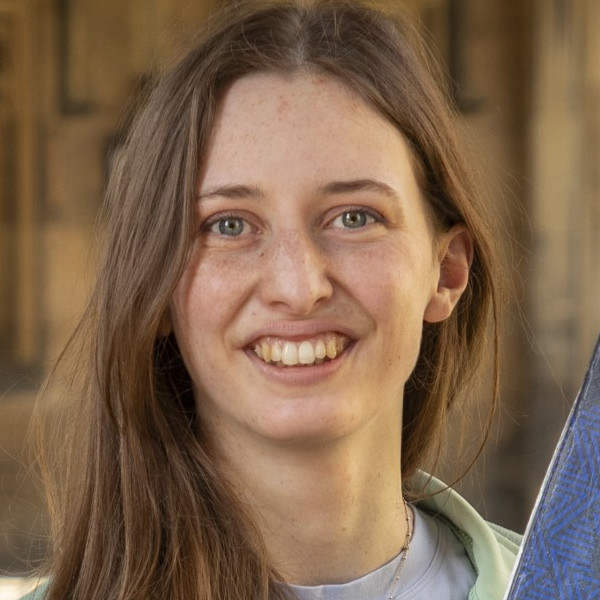
\includegraphics[width=0.09\textheight]{people/charlotte_priestley.jpg}%
        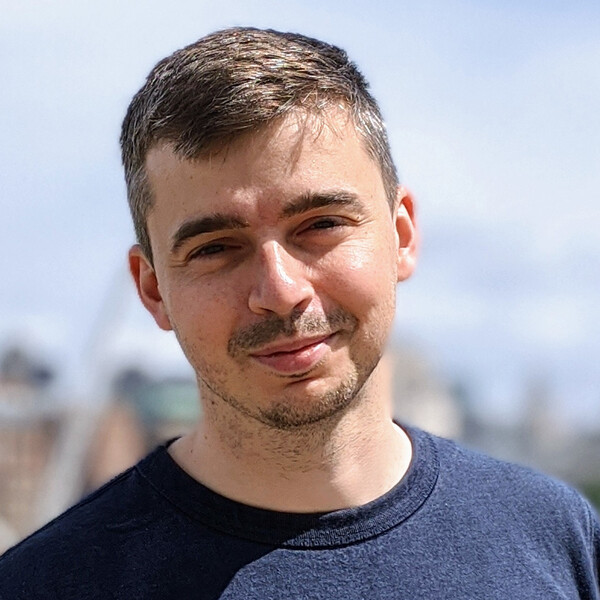
\includegraphics[width=0.09\textheight]{people/david_yallup.jpg}%
        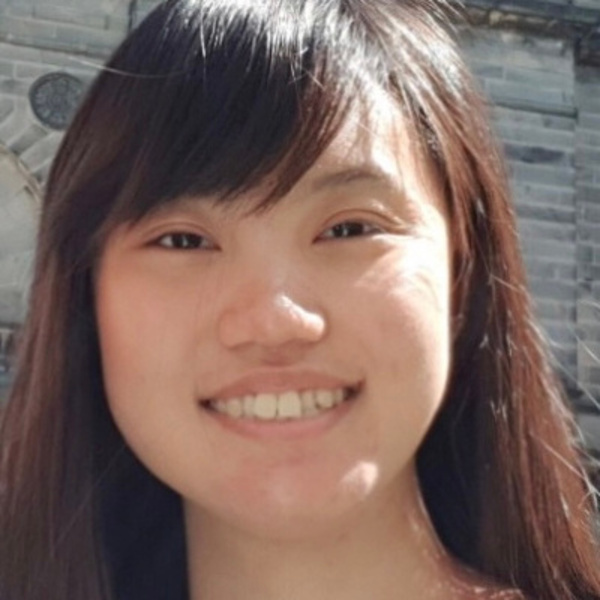
\includegraphics[width=0.09\textheight]{people/dily_ong.jpg}%
        
\includegraphics[width=0.09\textheight]{people/harry_bevins.jpg}%
        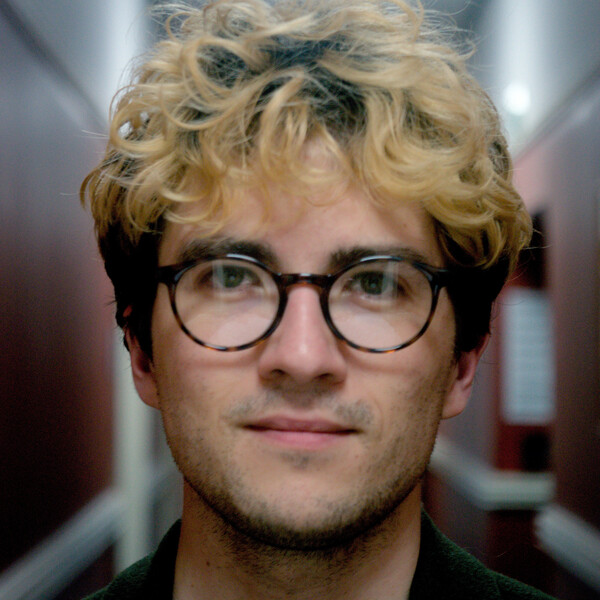
\includegraphics[width=0.09\textheight]{people/harvey_williams.jpg}%
        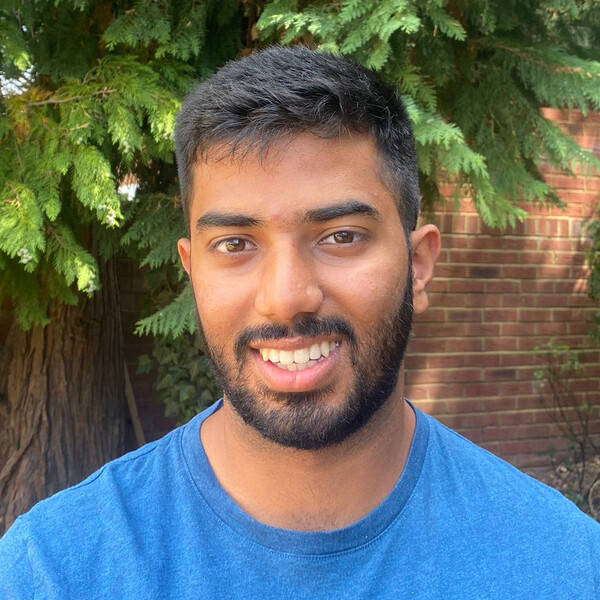
\includegraphics[width=0.09\textheight]{people/krish_nanavati.jpg}%
        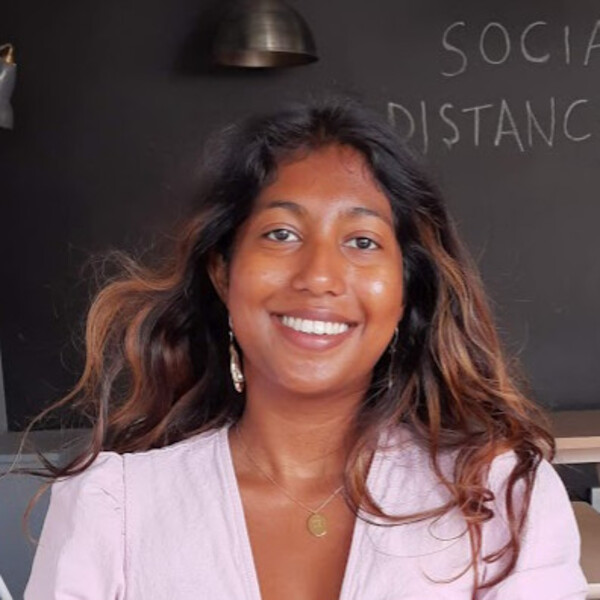
\includegraphics[width=0.09\textheight]{people/metha_prathaban.jpg}%
        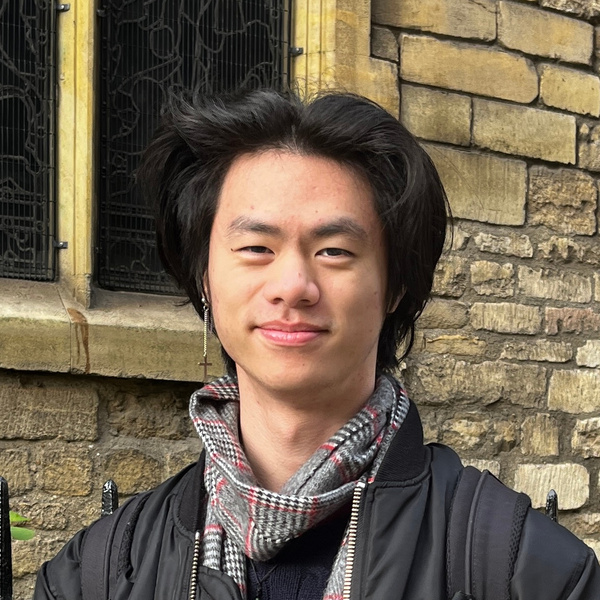
\includegraphics[width=0.09\textheight]{people/ming_yang.jpg}%
        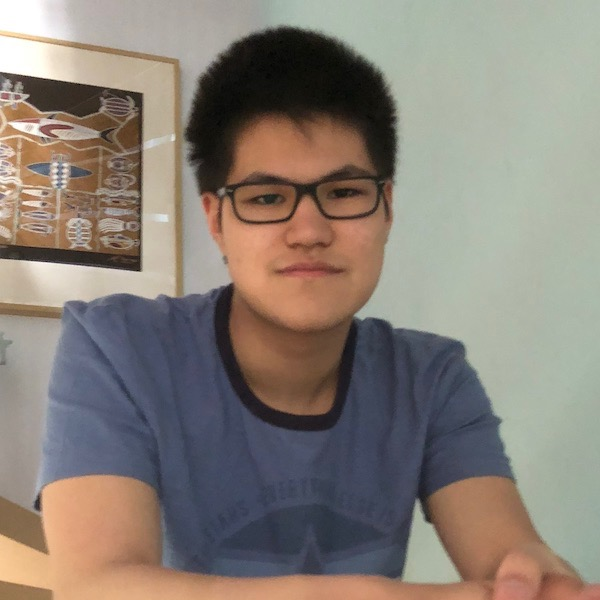
\includegraphics[width=0.09\textheight]{people/namu_kroupa.jpg}%
        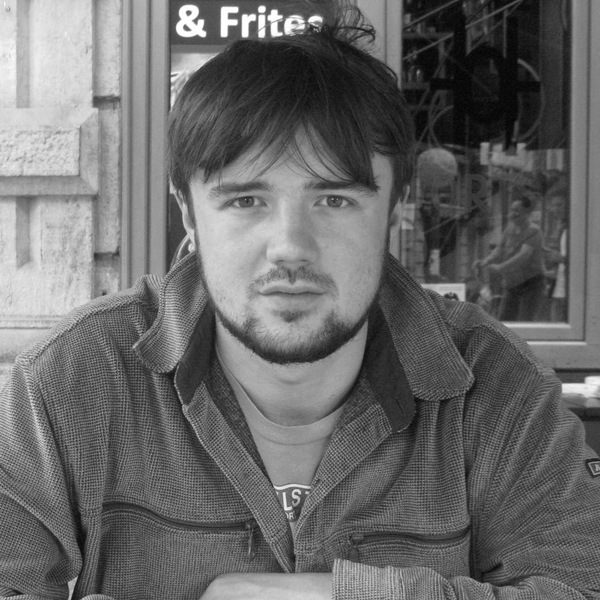
\includegraphics[width=0.09\textheight]{people/sam_leeney.jpg}%
        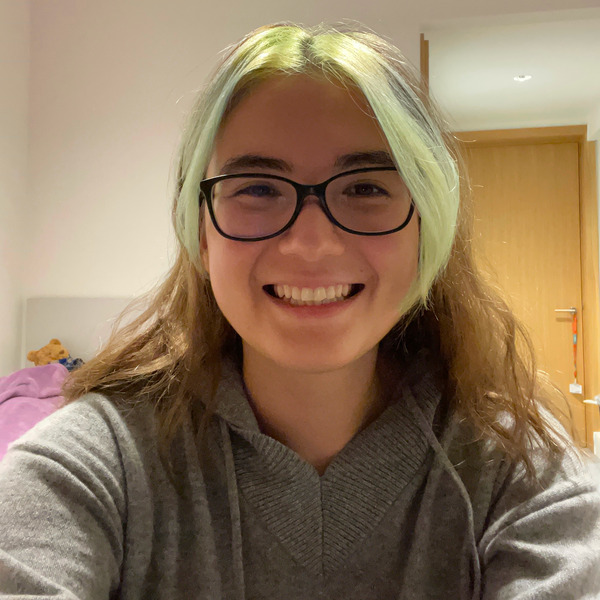
\includegraphics[width=0.09\textheight]{people/sinah_legner.jpg}%
        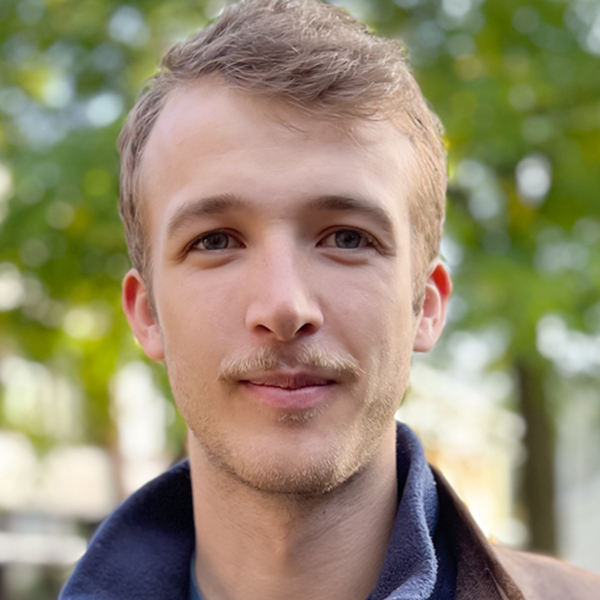
\includegraphics[width=0.09\textheight]{people/toby_lovick.jpg}%
        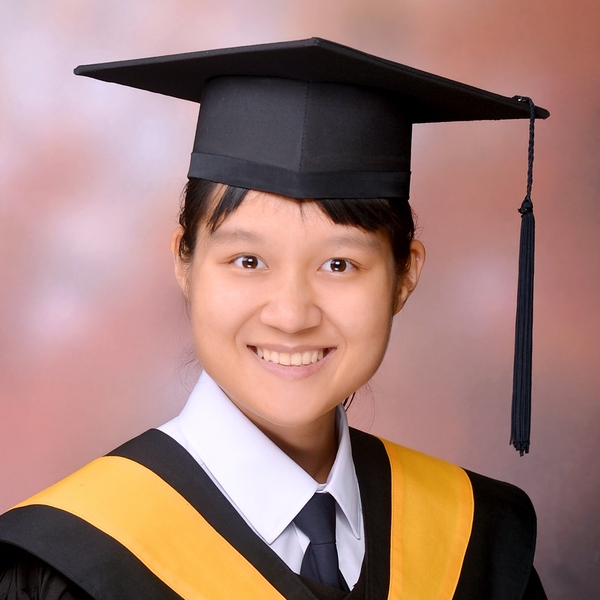
\includegraphics[width=0.09\textheight]{people/wei-ning_deng.jpg}%
        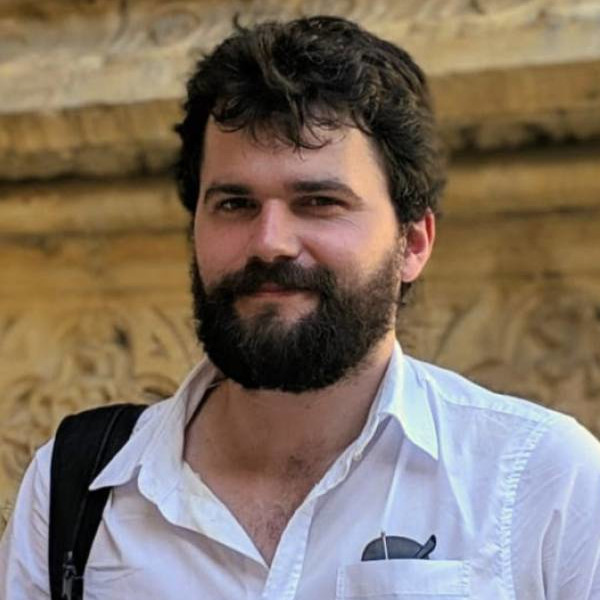
\includegraphics[width=0.09\textheight]{people/will_handley.jpg}%
        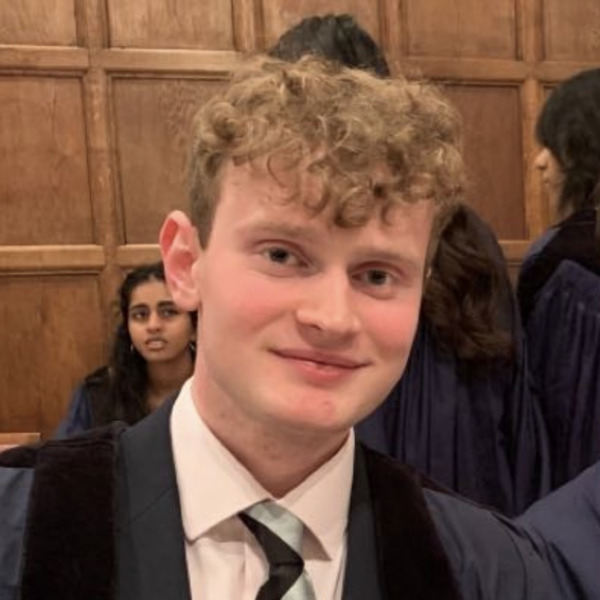
\includegraphics[width=0.09\textheight]{people/will_templeton.jpg}%
    };
    \begin{itemize}
        \item \textbf{Introduction to \texttt{lsbi}:} A linear simulation-based inference method developed over 18 months by the speaker and collaborators.
        \item \textbf{Benefits of Linear SBI:} Pedagogical value, practical examples with known ground truths, competitive accuracy, speed, and interpretability compared to neural networks.
        \item \textbf{Mathematical Setup:} Uses a linear generative model to fit simulation data and iteratively refine posterior estimations, demonstrated through toy and cosmology examples.
        \item \textbf{\texttt{lsbi} Python Package:} Extends \texttt{scipy.stats.multivariate\_normal} with functionalities for marginalization, conditioning, and plotting; under active development and open source.
        \item \textbf{Future Directions:} Include realistic CMB simulations, extend to other examples (BAO, SNe), explore parameter limits, mixture modeling, and integrate importance sampling and model comparison.
    \end{itemize}
\end{frame}

\end{document}
